\documentclass[border=2pt]{standalone}
\usepackage{tikz}
\usepackage{amsmath}
\DeclareMathOperator{\rank}{rank}
\begin{document}
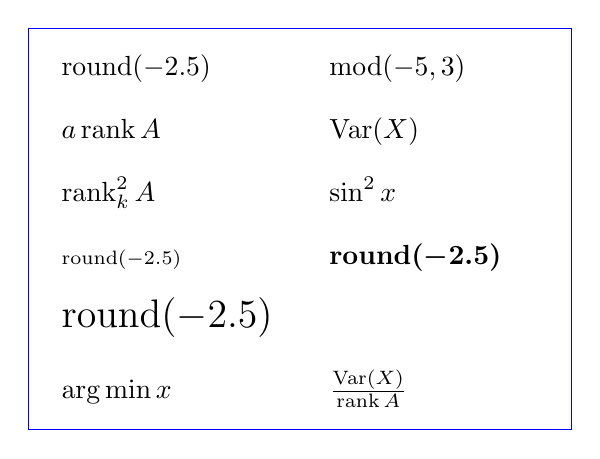
\begin{tikzpicture}
  \draw[blue] (-.3,.6) rectangle (6.6,-4.5);
  \node[anchor=base west] at (0,0) {$\operatorname{round}(-2.5)$};
  \node[anchor=base west] at (3.4,0) {$\operatorname{mod}(-5,3)$};
  \node[anchor=base west] at (0,-.8) {$a\rank A$};
  \node[anchor=base west] at (3.4,-.8) {$\operatorname{Var}(X)$};
  \node[anchor=base west] at (0,-1.6) {$\operatorname{rank}^2_k A$};
  \node[anchor=base west] at (3.4,-1.6) {$\sin^2 x$};
  \node[anchor=base west,font=\scriptsize] at (0,-2.4) {$\operatorname{round}(-2.5)$};
  \node[anchor=base west,font=\boldmath] at (3.4,-2.4) {$\operatorname{round}(-2.5)$};
  \node[anchor=base west,font=\Large] at (0,-3.2) {$\operatorname{round}(-2.5)$};
  \node[anchor=base west] at (0,-4.1) {$\operatorname{arg\,min} x$};
  \node[anchor=base west] at (3.4,-4.1) {$\frac{\operatorname{Var}(X)}{\operatorname{rank} A}$};
\end{tikzpicture}
\end{document}
